\documentclass{../source/Experiment}

\major{信息工程}
\name{姚桂涛}
\title{小信号调谐放大器}
\expname{小信号调谐放大器}
\stuid{3190105597}
\college{信息与电子工程学院}
\date{\today}
\lab{东4-319}
\course{通信原理实验}
\instructor{金向东、龚淑君}
\grades{}
\exptype{验证性实验}
\partner{叶慷鹏}
\begin{document}
\section{实验目的和要求}
    (1)掌握小信号调谐放大器的工作原理。

    (2)掌握频谱分析仪的基本使用方法。

    (3)掌握调谐放大器电压增益、通频带及选择性的定义、测试及计算方法。

    \section{实验原理}
    小信号调谐放大器广泛用作高频和中频放大器,特别是用在通信接收端的前端电路,其主要目的就是实现对高频小信号的放大。

    小信号调谐放大器的幅频特性:
    \begin{figure}[H]
        \centering
        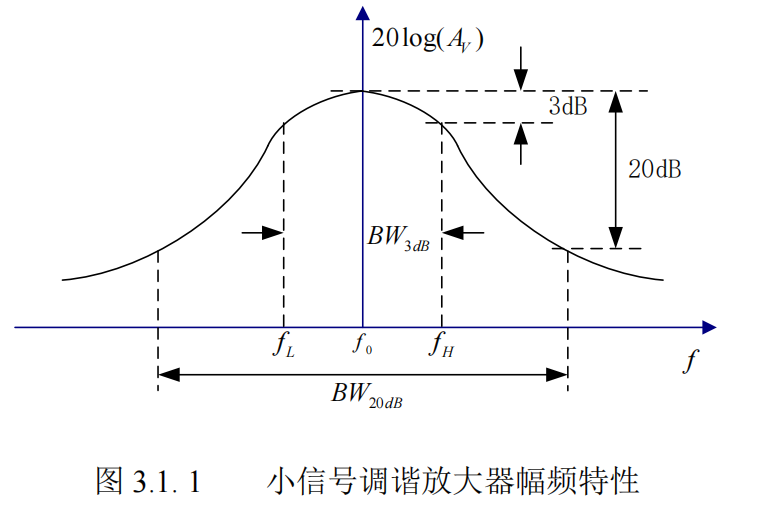
\includegraphics[scale=0.4]{figure/fig1.png}
    \end{figure}

    调谐放大器特性测试采用扫频法,采用带跟踪源的频谱仪进行测试。

\end{document}